% ======================================================================

\chapter{Raceline Optimization}
\label{chap:opt}

Lo studio di questa tesi si è concentrato a trovare una soluzione al seguente problema:\
\textit{trovare la raceline globale ottima \emph{\footnotesize -- secondo un criterio scelto --} data una mappa}.
Il criterio di ottimizzazione principale, in questi casi, è il tempo di percorrenza del tracciato, ovvero
il \textit{laptime}.

Le porzioni interessanti di un circuito da gara sono le curve: ne esistono di diversi tipi e altrettanti
modi per affrontarle in base al tipo; trovare una percorso ottimo, in questo senso, è un compito complesso e
il percorso più breve non implica quello col minor tempo per via, appunto, delle curve, che riducono la
velocità media. Dunque una strategia migliore è quella di trovare la traiettoria con le curvature minori,
così da mantenere una velocità più alta nell'affrontarle. Anche questo approccio, tuttavia, non prende in
considerazione una sequenza di curve e la velocità di uscita da una curva. Il percorso ottimo in termini
di tempo, quindi, è un compromesso tra queste due strategie, ovvero quello che minimizza la distanza
percorsa mantenendo alta la velocità nelle curve ed eventualmente anche in uscita da esse.

É bene precisare che la traiettoria generata è ottima \textbf{solo} nel contesto considerato, ovvero
quello di un singolo robot sul tracciato, senza alcun rivale. È da considerare un'operazione preliminare
alla gara, perchè si ha necessità di conoscere la mappa.
Tuttavia non è utile solo nel contesto considerato: la raceline ottima, avendo una visione globale sulla
mappa, può essere sfruttata da un local o behavioural planner come linea guida.

\section{Le curve}
Il fulcro di cui l'ottimizzazione si occupa è come affrontare le curve.\\
Caratteristica principale di una curva è il suo raggio: un raggio maggiore corrisponde a velocità più alte
e viceversa; inoltre, si distinguono il raggio esterno e quello interno e la loro differenza risulta
nell'ampiezza della curva.
Esistono anche caratteristiche di natura tridimensionale, come la variazione dell'altezza e
l'inclinazione, tuttavia non sono state oggetto di studio in questa tesi dal fatto che il contesto di
f1tenth non include questa variabilità, come accade nelle gare di F1.

In linea generale, una curva può essere suddivisa in quattro sequenze principali: %, come mostrato in figura:%TODO: ref
\begin{enumerate}
	\item Approccio e decelazione
	\item Inizio della curva
	\item Apice
	\item Uscita della curva e accelerazione
\end{enumerate}

Anche la traiettoria, dato che segue una curva, può essere definita con un raggio che può essere
costante o variabile dall'inzio della curva fino alla fine.

\begin{figure}[h]
	\begin{center}
		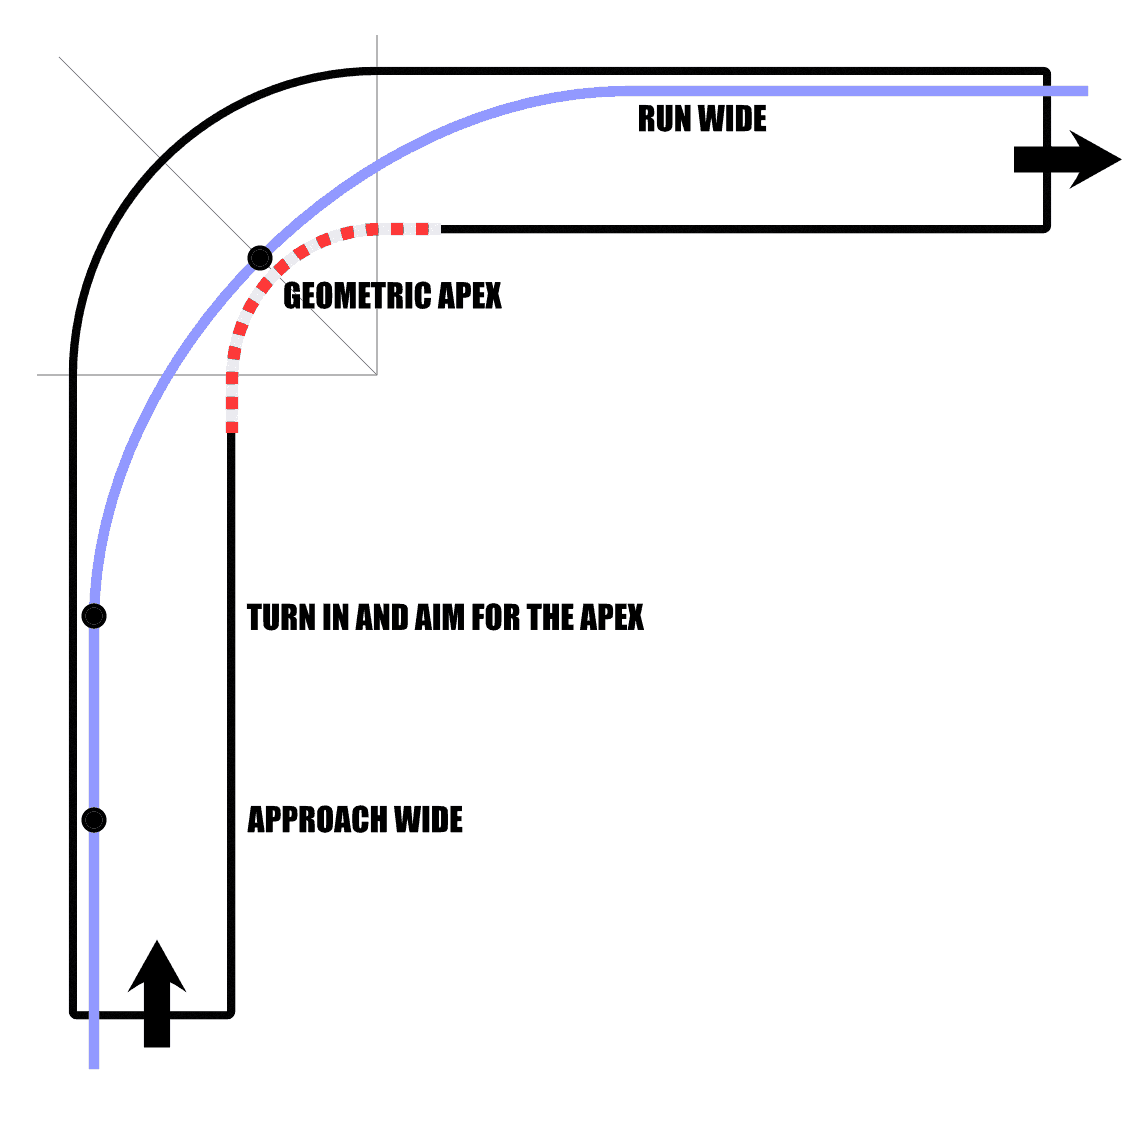
\includegraphics[width=0.65\textwidth]{geometric-apex.png}
	\end{center}
	\caption{Rappresentazione delle fase di una raceline geometrica per una curva a destra}\label{fig:geom-raceline}
\end{figure}

\paragraph{Raceline geometrica}
L'approccio più semplice e immediato per affrontare una curva genera una raceline che prende il
nome di \textit{raceline geometrica}. La strategia prevedere queste sequenze, rappresentate in figura
\ref{fig:geom-raceline}:
\begin{enumerate}
	\item Approccio largo e verso l'esterno del circuito 
	\item Sterzata verso il centro del raggio interno della curva 
	\item Uscita larga e verso l'esterno del circuito
\end{enumerate}
Si tratta, quindi, di una raceline a raggio costante.\\
I principali vantaggi di questo approccio rispetto alla raceline ottima sono la sua semplicità, sia in
termini di esecuzione sia in termini di computazione, e la possibilità di mantenere un'alta velocità
durante la curva. Tuttavia, la raceline geometrica ha importanti svantaggi quali una decelazione
prematura all'entrata della curva, una accelerazione ritardata all'uscita e la possibilità di essere in
uno stato svantaggiato per affrontare la prossima curva, nel caso di curve in sequenza.

Dunque, la raceline ottimale non dovrebbe tener conto solamente della singola curva ma eventualmente
anche di quelle successive: per estensione, quindi, deve essere considerato tutto il circuito.

\paragraph{Raceline ottimale}
Al contrario della raceline geometrica, non è possibile definire a priori le sequenze da seguire come
fatto in precedenza, proprio perchè dipende dalle caratteristiche della curva.
Riprendendo come esempio la curva in figura \ref{fig:geom-raceline}, la raceline ottimale, ovvero quella
che riesce ad eseguire la curva nel minor tempo possibile, tarda il più possibile l'inizio della curva
per mantenere più velocità all'entrata, decelera più velocemente e ha una virata più stretta e con un
apice più distante da quello geometrico, così facendo si ha la possibilità di aver più tempo per
accelerare di nuovo all'uscita della curva con la possibità di mantenere una traiettoria più centrata
rispetto al circuito.

In figura \ref{fig:cmp-lines} vi è una comparazione grafica tra le due raceline.\\
La raceline ottima, inoltre, adegua la traiettoria di uscita in base alla curva successiva, se presente,
in modo tale da affrontarla anch'essa nel modo ottimale. Si nota la distinzione in figura
\ref{fig:cmp-opt-lines}.

\begin{figure}[h]
	\begin{minipage}[c]{0.45\textwidth}
		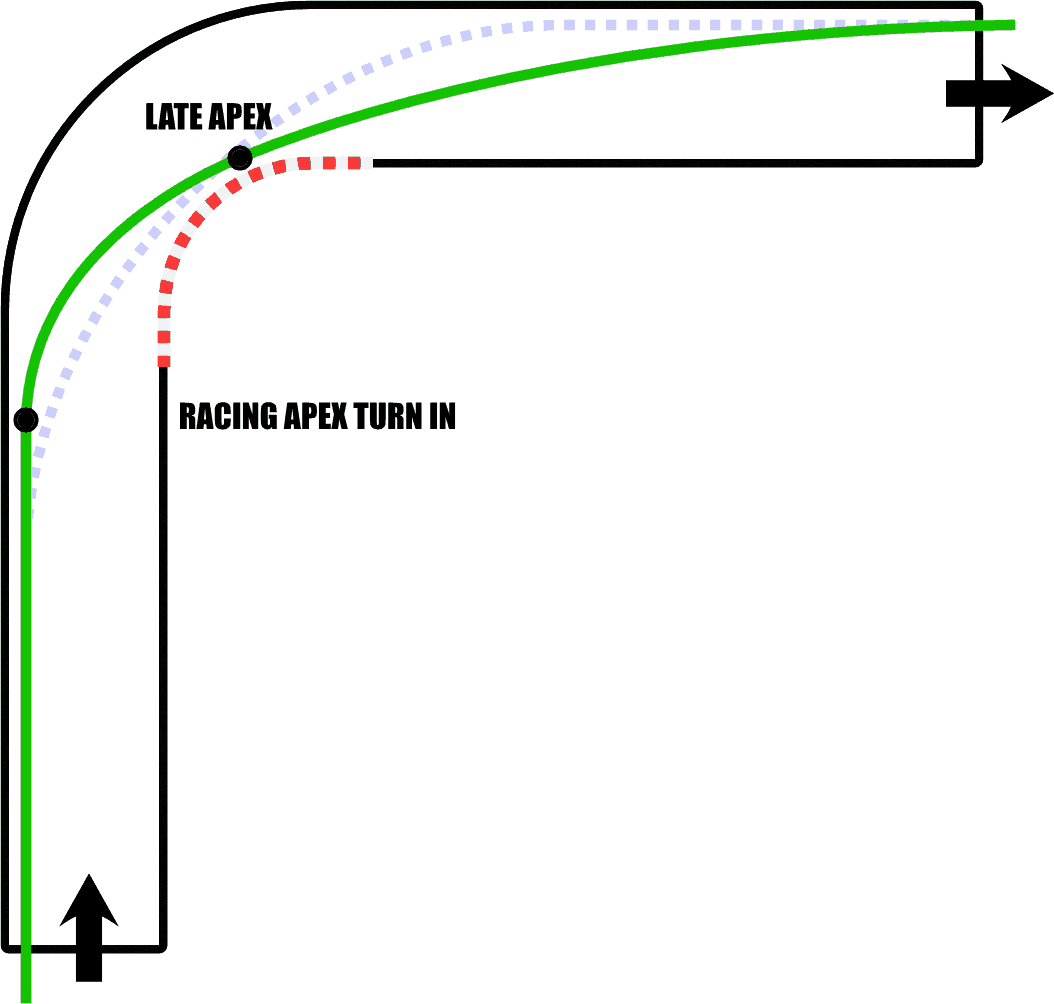
\includegraphics[width=0.80\textwidth]{comparing-lines.png}
		\caption{Comparazione tra raceline ottimale, in verde, e raceline geometrica, in blu tratteggiato}\label{fig:cmp-lines}
	\end{minipage}\hfill
	\begin{minipage}[c]{0.45\textwidth}
		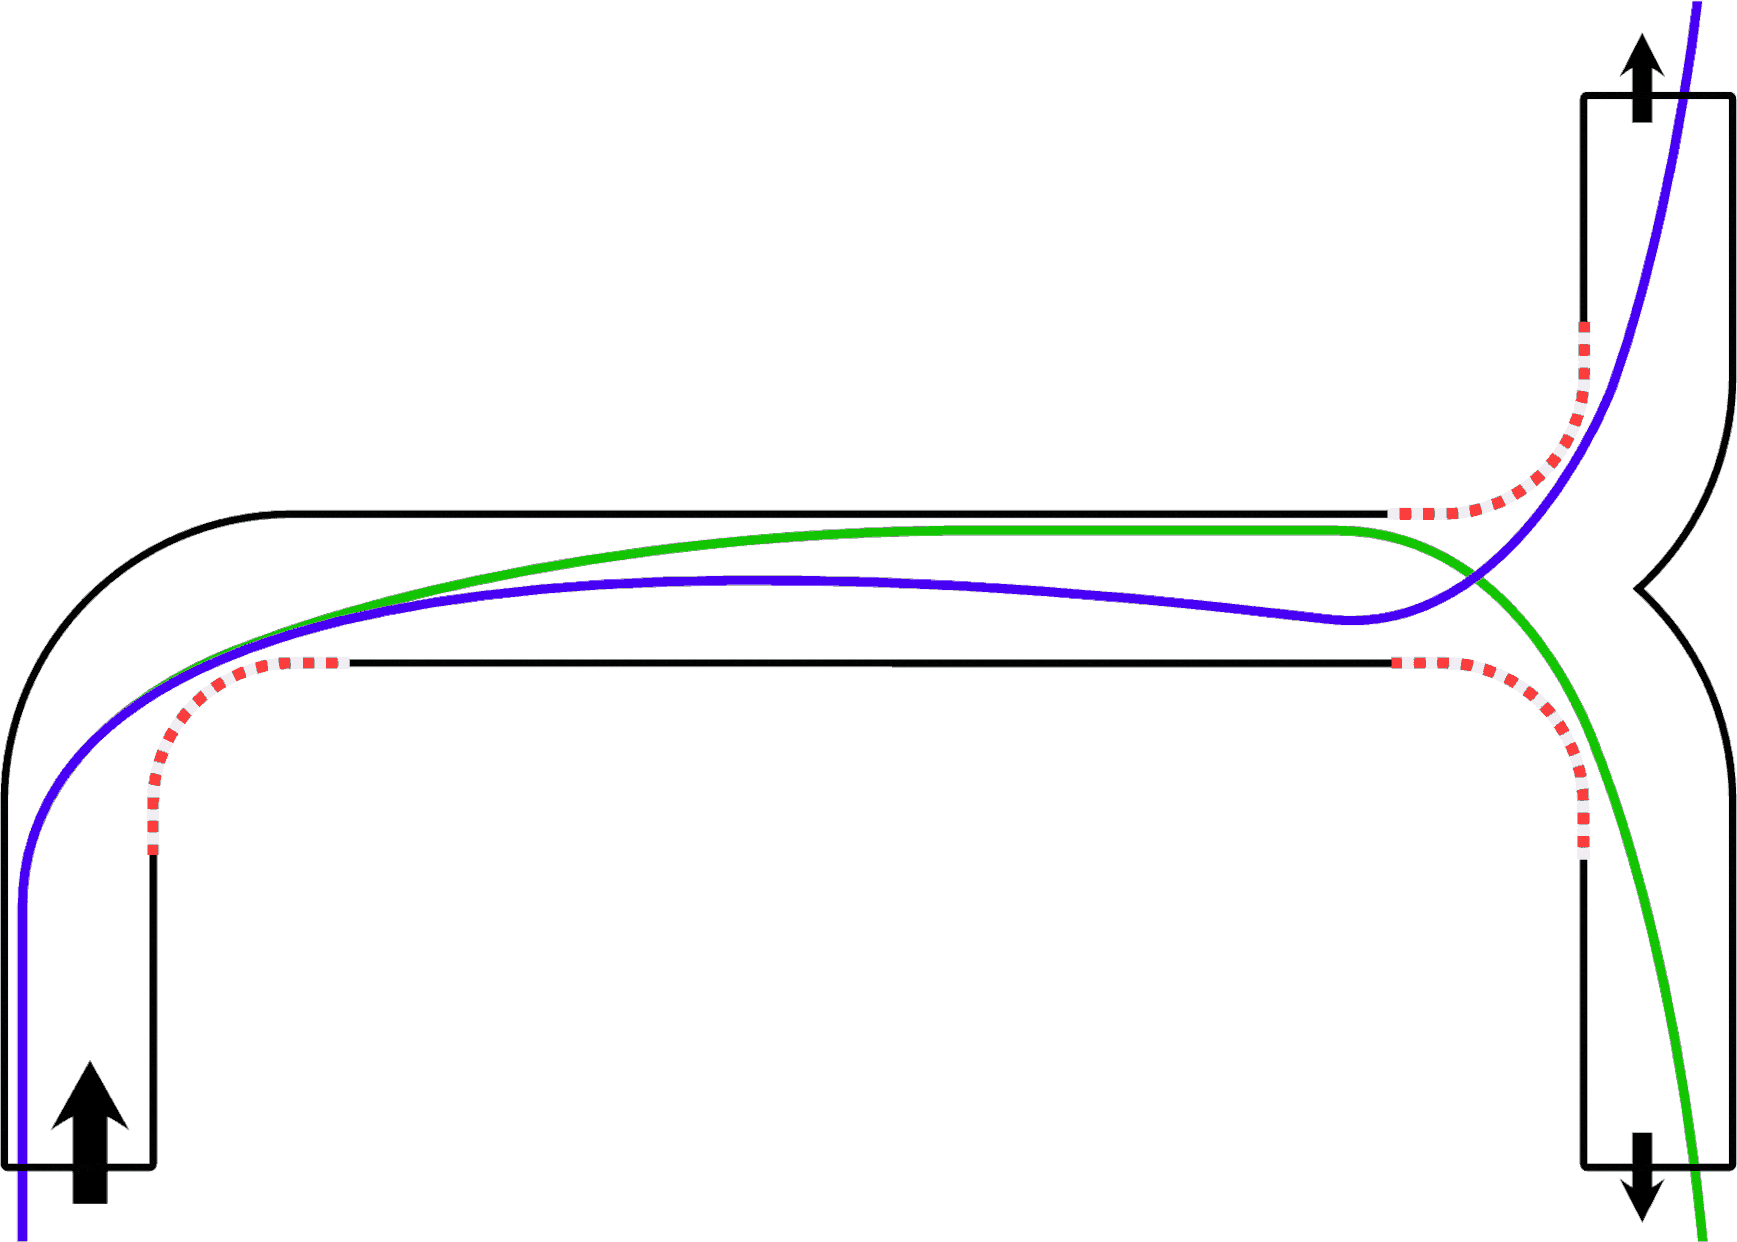
\includegraphics[width=1\textwidth]{multiple-corners.png}
		\caption{Confronto tra raceline ottime con due curve in sequenza}\label{fig:cmp-opt-lines}
	\end{minipage}
\end{figure}


\section{Processo di generazione}

% Il lavoro è stato basato su questa repo \url{https://github.com/CL2-UWaterloo/Raceline-Optimization}.
%
% Il processo, ad alto livello, si può riassumere nei seguenti passaggi:
% \begin{enumerate}
% 	\setlength\itemsep{0em}
% 	\item Si genera una occupancy grid di un circuito 
% 	\item Si genera la centerline, ovvero si calcola la larghezza del tracciato 
% 	\item Si genera la traiettoria
% \end{enumerate}
%
% % ===== Definizione di centerline ======================================
% Il tracciato deve essere discretizzato per poter essere computato da una macchina.
% L'idea, quindi, è quella di considerare la linea che si trova esattamente a metà della larghezza della
% porzione di circuito presa in considerazione; questa linea viene poi discretizzata prendendone un punto
% ad egual distanza l'uno dall'altro -- chiamati \textit{samples}.
% È utile, nella descrizione matematica del problema, che i samples non siano semplici punti descritti
% dalle coordinate in un piano cartesiano, ma siano dei vettori con una direzione, ovvero quella della
% gara: un sample punterà verso il sample successivo.
% % TODO: parlare della generazionel della centerline
%
% % ===== Definizione della raceline =====================================
% Dati i samples della centerline, i punti che formano la raceline giacciono sulla linea immaginaria
% ortogonale alla centerline che unisce il sample della centerline con gli bordi del circuito.\\
% Come lo sono i sample della linea di riferimento, anche la raceline è definita come vettori che puntano
% l'uno al successivo. \\
% Dunque è possibile definire la raceline con la seguente formula
% \[
% 	\overrightarrow{r_i} = \overrightarrow{p_i} + \alpha_i \overrightarrow{n_i}
% \]
% ovvero, il vettore 
